%&pdflatex
\section{Selezione del software}
L'ultimo passaggio riguarda l'installazione di software aggiuntivo su Debian. Possiamo scegliere se installare un \textit{desktop environment} (ambiente desktop) e quale installare; se vogliamo installare un \textit{web server}, un \textit{server di stampa} (\texttt{cups}), un \textit{server ssh} e le utility di base per l'amministrazione del sistema.

Il desktop environment è l'ambiente grafico. Se non scegliamo nessun desktop environment ci ritroveremo con un sistema operativo con la sola linea di comando (terminale) dove poter digitare comandi uno per volta. Per installare un desktop environment, dobbiamo selezionare la voce \texttt{Debian desktop environment} (\texttt{Ambiente desktop Debian}) e una (e una soltanto) delle voci sottostanti (\texttt{GNOME}, \texttt{Xfce}, \texttt{KDE}, \texttt{Cinnamon}, \texttt{MATE}, \texttt{LXDE}). La scelta, va fatta in base alle proprie preferenze. Di seguito, elenchiamo alcune caratteristiche di ognuno di questi desktop environment:
\begin{itemize}
	\item \textbf{GNOME} è il desktop environment più utilizzato al mondo. Ha come scopo l'usabilità e l'immediatezza d'uso, senza rinunciare all'estetica. Contiene molti programmi preinstallati;
	\item \textbf{Xfce} è un desktop environment minimale e leggero, adatto a chi preferisce un desktop environment essenziale e funzionale;
	\item \textbf{KDE} è un desktop environment molto potente e personalizzabile, ma anche molto pesante. Contiene molti programmi preinstallati;
	\item \textbf{Cinnamon} è il desktop environment prodotto dagli sviluppatori di \textit{Linux Mint}. Derivato di \texttt{GNOME}, è pensato per essere comodo e facile da usare;
	\item \textbf{MATE} è un desktop environment derivato dal codice di \texttt{GNOME 2} non più mantenuto dopo il rilascio della versione 3. È nato nel 2011 per iniziativa di alcuni membri della comunità di \textit{Arch Linux};
	\item \textbf{LXDE} Ambiente desktop minimale e veloce, ma con una grafica più accattivante di Xfce. Non è però più mantenuto, in quanto è stato rimpiazzato da \texttt{LXQT}.
\end{itemize}
Si consiglia al lettore di cercare con il proprio motore di ricerca preferito immagini riguardo ad ognuno di questi ambienti: può, in questo modo, farsi un'idea dell'aspetto grafico di questi desktop environment.

Il \textit{web server} non ci serve: è utile solo se vogliamo installare Debian su un server che dovrà ospitare un sito web. Non ci serve neanche il \textit{server SSH} che viene utilizzato per l'accesso remoto al sistema. Il \textit{print server} (server di stampa) è utile se vogliamo poter stampare documenti con una stampante da Debian. Infine, è consigliato installare le utility di sistema che servono a configurare e gestire al meglio il proprio ambiente.

Una possibile configurazione, dove viene installato Xfce come desktop environment, è quella mostrata in Figura \vref{fig:software-selection}. Dopo aver fatto avanti, l'installer inizierà a scaricare il software che abbiamo selezionato.

\begin{figure}[ht]
	\centering
	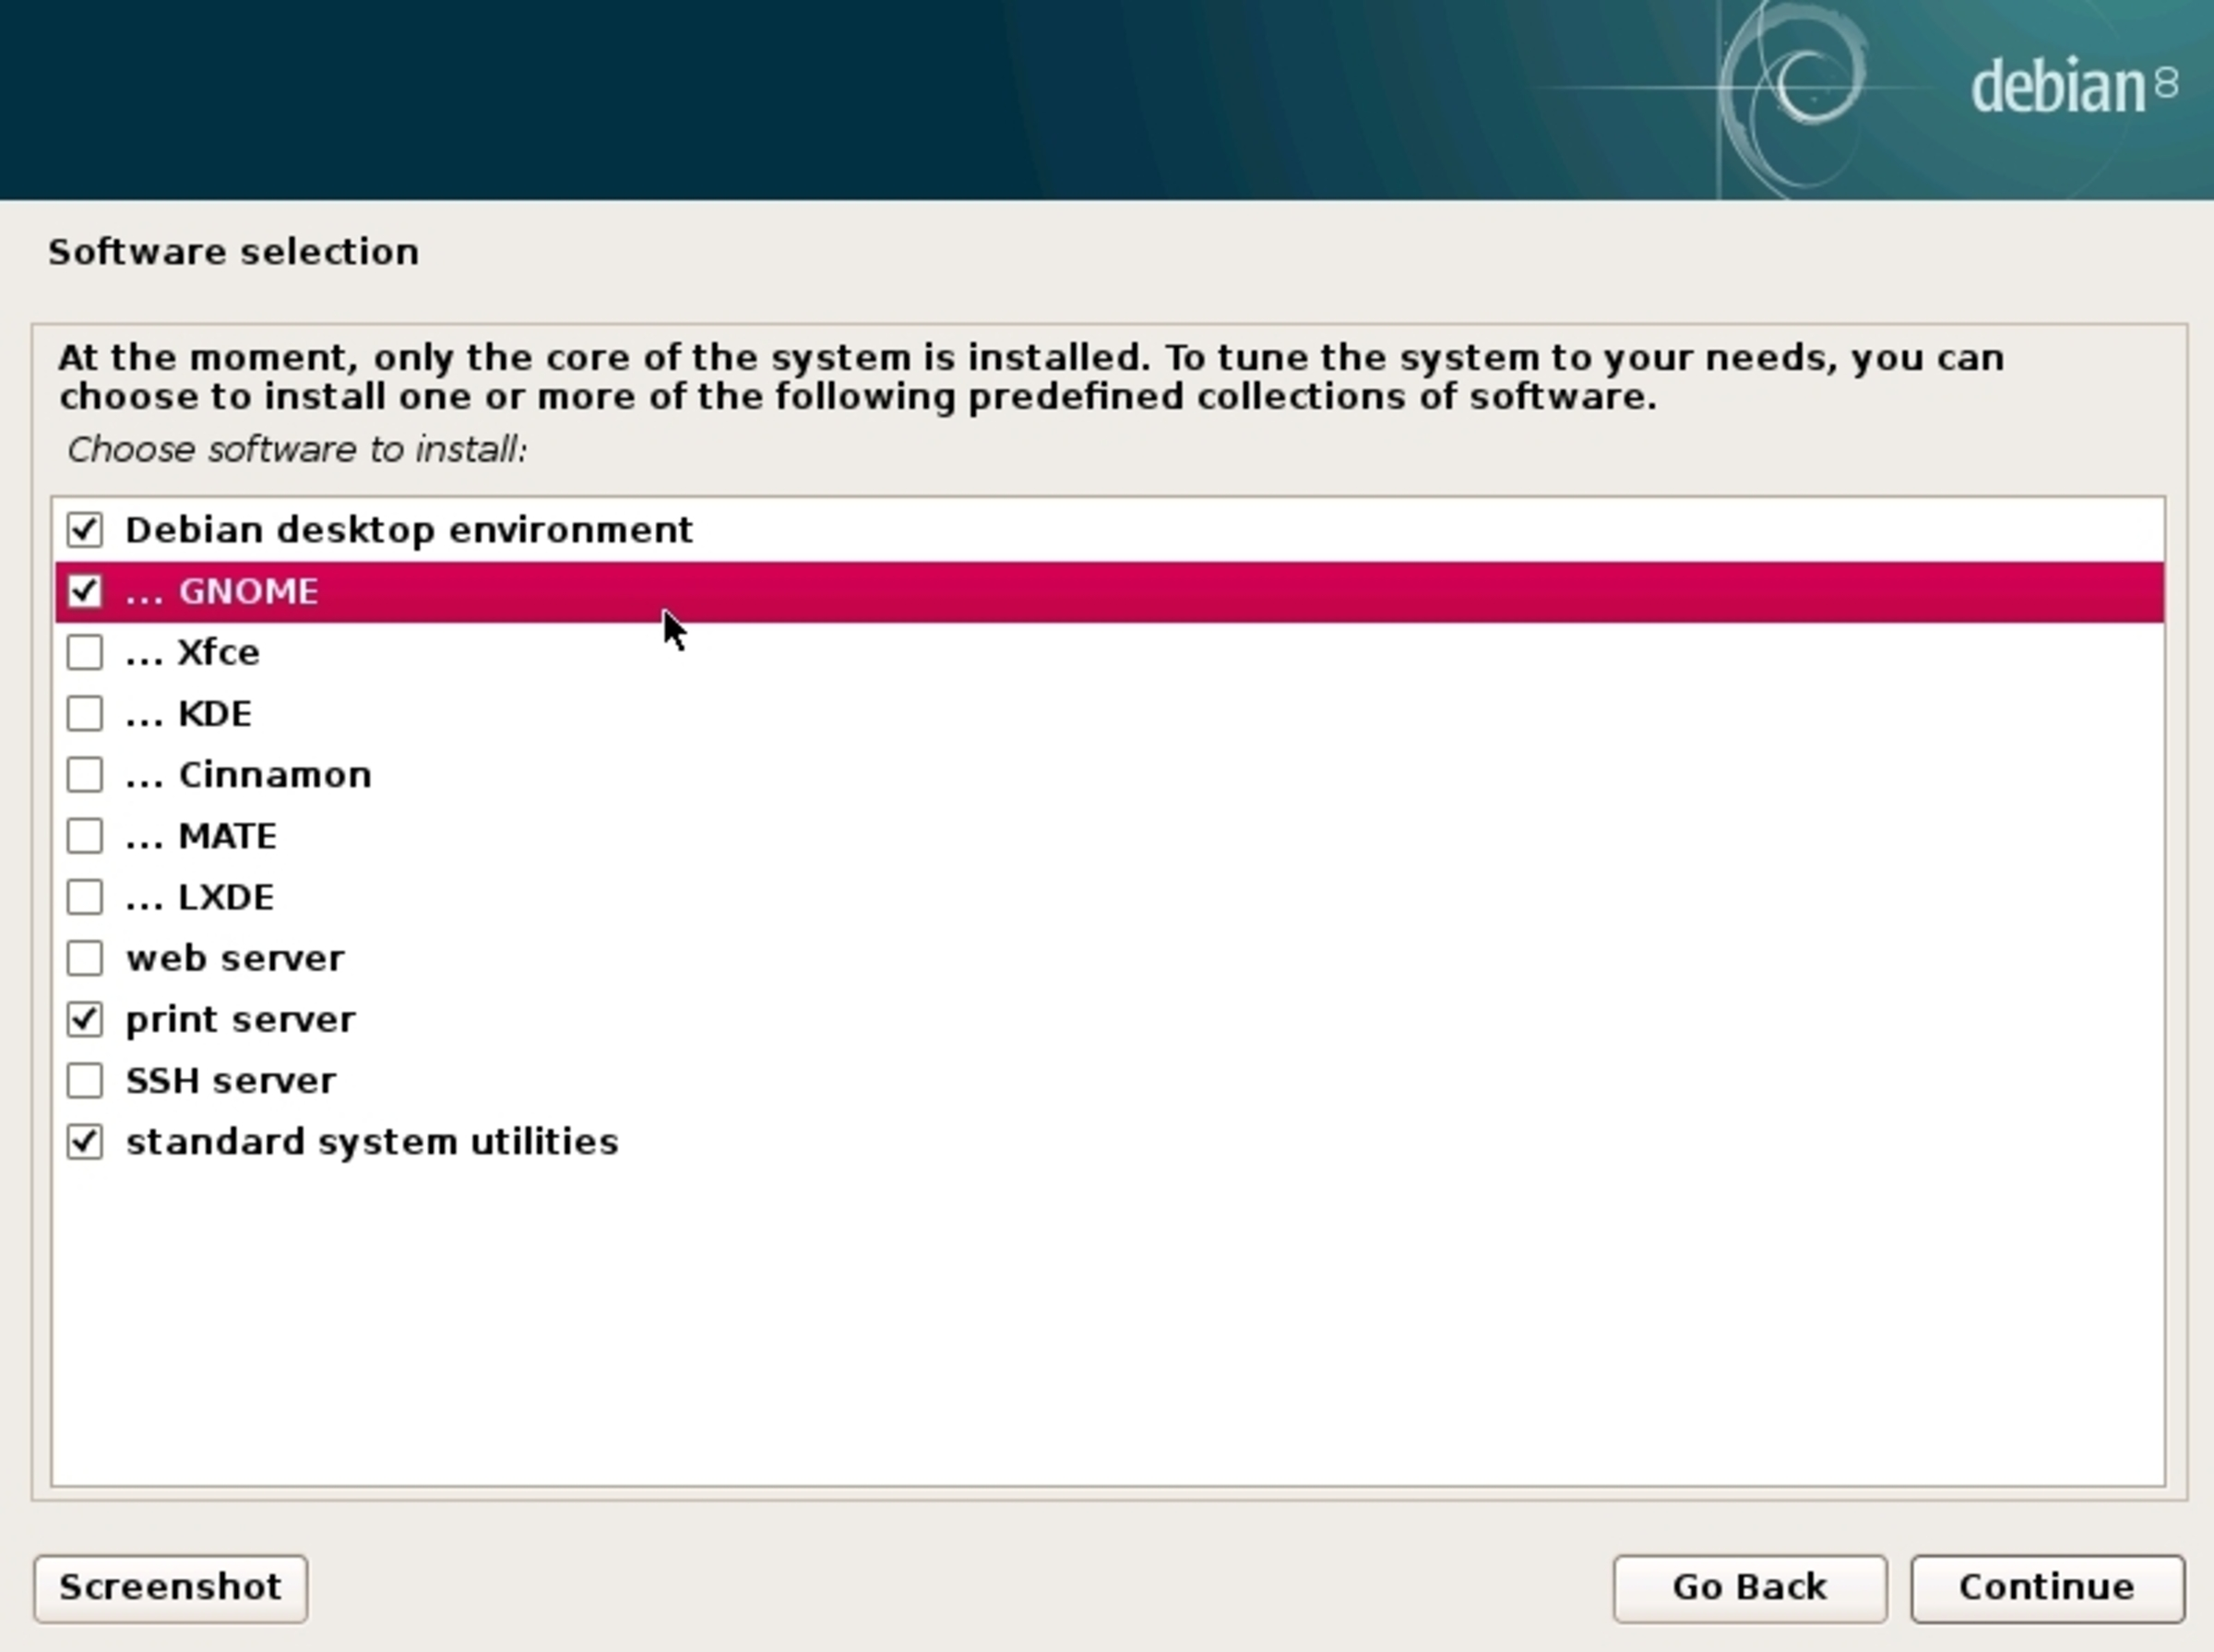
\includegraphics[resolution=600]{software-selection}
	\caption{Scelta del software e di Xfce come desktop environment}
	\label{fig:software-selection}
\end{figure}
